\subsection{Artinian Rings and Noetherian Rings}

DEFINITION 2. --- A ring A is said to be left Artinian (resp. left Noetherian) if the left A-module \(A_{s}\) is Artinian (resp. Noetherian). Likewise, a ring A is said to be right Artinian (resp. right Noetherian) if the right A-module \(A_{d}\) is Artinian (resp. Noetherian).

A ring A is right Artinian (resp. right Noetherian) if and only if its opposite ring \(A^{o}\) is left Artinian (resp. left Noetherian). For a commutative ring A, the properties of being left Artinian and of being right Artinian coincide, and when they are hold, we say that the ring A is Artinian; we adopt an analogous convention for ``Noetherian.'' There exist noncommutative rings that are left Artinian but not right Artinian, and noncommutative rings that are left Noetherian but not right Noetherian (VIII, p.~14, Exercise 3).

Let \(A\) be a ring. By definition, the following properties are equivalent:

\begin{enumerate}
\def\labelenumi{(\roman{enumi})}
\item
  The ring A is left Artinian.
\item
  Every nonempty set of left ideals of A, ordered by inclusion, has a minimal element.
\item
  Every decreasing sequence of left ideals of A is stationary.
\end{enumerate}

Because of Proposition 2 of VIII, p.~3, the following properties are equivalent:

\begin{enumerate}
\def\labelenumi{(\roman{enumi})}
\item
  The ring A is left Noetherian.
\item
  Every nonempty set of left ideals of A, ordered by inclusion, has a maximal element.
\item
  Every increasing sequence of left ideals of A is stationary.
\item
  Every left ideal of A is generated by a finite subset of A.
\end{enumerate}

Examples. --- 1) A field is a ring that is both left and right Artinian and Noetherian.

\begin{enumerate}
\def\labelenumi{\arabic{enumi})}
\setcounter{enumi}{1}
\item
  Let A be a ring and D a subring of A. Suppose that D is a field and that A is a finite-dimensional left vector space over D. Then the ring A is left Artinian and left Noetherian because every left ideal of A is a D-vector subspace of A. In particular, a finite-dimensional algebra over a commutative field is a ring that is both left and right Artinian and Noetherian.
\item
  A principal ideal domain (VII, §1, No.~1, p.~1, Definition 1) is Noetherian. An integral domain A that is not a field is not an Artinian ring: for every nonzero noninvertible element \(a\) of A, the sequence of ideals \(a^n\mathbf{A}\) (for \(n \in \mathbf{N}\) ) is strictly decreasing. In particular, the ring \(\mathbf{Z}\) of integers is Noetherian but not Artinian.
\item
  Let M be an A-module that is the direct sum of an infinite family \((\mathrm{M}_{i})_{i\in\mathrm{I}}\) of nonzero submodules. Let E be the endomorphism ring of M. For every \(i\in I\) , let \(a_{i}\) (resp. \(b_{i}\) ) be the set of elements of E with kernel containing \(\sum_{j\neq i}M_{j}\) (resp. with image contained in \(M_{i}\) ). Then \((a_{i})\) is an infinite family of nonzero left ideals of E whose sum is direct, and \((b_{i})\) is an infinite family of nonzero right ideals of E whose sum is direct. Consequently, the ring E is neither left nor right Artinian (resp. Noetherian) (VIII, p.~2, Example 2). In particular, the endomorphism ring of an infinite-dimensional vector space is neither left nor right Artinian (resp. Noetherian).
\end{enumerate}

THEOREM 1. --- Let A be a left Artinian ring. The A-module \(A_{s}\) has finite length.

We will use the following lemma in the proof.

Lemma 3. --- Let A be a ring and n a natural number. An Artinian A-module M that is the sum of a family of submodules of length \(\leqslant n\) has finite length.

We use induction on n.~First, suppose n = 1. If M were not of finite length, then we could construct a sequence \((\mathrm{M}_{m})_{m \in \mathbf{N}}\) of submodules of M of length 1 with \(M_{m} \not\subset (\sum_{i < m} M_{i})\) for every \(m \in N\) . We would then have \(M_{m} \cap \sum_{i < m} M_{i} = 0\) for every m, and the sum of the family \((\mathrm{M}_{m})_{m \in \mathbf{N}}\) would be direct. However, this contradicts the fact that the A-module M is Artinian (VIII, p.~2, Example 2).

Now, suppose \(n \geqslant 2\) . Let \((\mathrm{M}_{i})_{i \in \mathrm{I}}\) be a family of submodules of M of length \(\leqslant n\) with sum M. For every \(i \in I\) , choose a submodule \(M_{i}^{\prime}\) of \(M_{i}\) of length \(\leqslant n - 1\) such that \(M_{i}/M_{i}^{\prime}\) has length \(\leqslant 1\) . Set \(M^{\prime} = \sum M_{i}^{\prime}\) , and denote the image of \(M_{i}\) in \(M^{\prime\prime} = M/M^{\prime}\) by \(M_{i}^{\prime\prime}\) . The modules \(M_{i}^{\prime\prime}\) are of length \(\leqslant 1\) , and their sum is \(M^{\prime\prime}\) . The modules \(M^{\prime}\) and \(M^{\prime\prime}\) are Artinian (VIII, p.~3, Proposition 3); by the induction hypothesis, they are of finite length. Hence, M has finite length (II, §1, No.~10, p.~212, Proposition 16).

Let us now prove Theorem 1. Let S denote the set of left ideals a of A such that the module \(A_{s}/a\) has finite length. Let \((\mathfrak{a}_{i})_{i\in I}\) be a finite family of elements of S. By Proposition 1 of VIII, p.~2, the A-module \(A_{s}/a_{i}\) is Artinian and Noetherian for every \(i\in I\) . Consequently, \(A_{s}/\bigcap_{i\in I}a_{i}\) is Artinian and Noetherian (VIII, p.~4, Corollary of Proposition 3), hence of finite length (VIII, p.~2, Proposition 1). This proves that S is a left directed set for the inclusion. Since the ring A is left Artinian, the set S has a least element b. We denote the length of the A-module \(A_{s}/b\) by n.

Let \(x\) be an element of \(A_s\) and \(\mathfrak{a}\) its annihilator (II, §1, No.~12, p.~219). The A-module \(Ax\) is isomorphic to \(A_s / \mathfrak{a}\) . If \(Ax\) has finite length, then \(\mathfrak{a}\) belongs to \(\mathscr{S}\) , so \(\mathfrak{a}\) contains \(\mathfrak{b}\) and \(Ax\) has length \(\leqslant n\) . Thus, every monogenous left ideal of \(A\) of finite length has length \(\leqslant n\) . Let \(\mathfrak{c}\) be the sum of these ideals; this is a left ideal of \(A\) , of finite length by Lemma 3. Every left ideal of \(A\) of finite length is a sum of monogenous left ideals of finite length and is therefore contained in \(\mathfrak{c}\) . Hence, \(\mathfrak{c}\) is the largest left ideal of \(A\) of finite length.

If c were distinct from A, then the set of left ideals of A containing c and distinct from c would have a minimal element \(c'\) . The A-module \(c'/c\) would then have length 1, and \(c'\) would have finite length, which contradicts the fact that c is maximal. We therefore have c = A; the A-module \(A_{s}\) has finite length.

COROLLARY. --- Every left Artinian ring is left Noetherian.

Let \(A\) be a left Artinian ring. By Theorem 1, the \(A\) -module \(A_s\) has finite length. We then apply Proposition 1 of VIII, p.~2.

Let A be a left (resp. right) Artinian ring; the length of the A-module \(A_{s}\) (resp. \(A_{d}\) ) (I, §4, No.~7, p.~44) is called the left (resp. right) length of the ring A. When A is a commutative Artinian ring, these two lengths coincide and are simply called the length of A. When A is left and right Artinian but is not commutative, the left and right lengths of A are not necessarily equal (VIII, p.~14, Exercise 3).

Example 5. --- The left and right lengths of a field are equal to 1.

PROPOSITION 4. --- a) Let A be a left Noetherian ring and M a finitely generated left A-module. The module M is Noetherian, and every submodule of M is finitely generated.

\begin{enumerate}
\def\labelenumi{\alph{enumi})}
\setcounter{enumi}{1}
\tightlist
\item
  Let A be a left Artinian ring and M a left A-module. The following properties are equivalent: the module M is finitely generated; the module M is Artinian; the module M has finite length; the module M is Noetherian.
\end{enumerate}

Let us prove a). Every monogenous submodule of M is isomorphic to a quotient of \(A_{s}\) , hence is Noetherian by Proposition 3 of VIII, p.~3. The module M is a finite sum of such submodules; it is therefore Noetherian by the corollary (VIII, p.~4) of Proposition 3. Every submodule of M is then finitely generated (VIII, p.~3, Proposition 2)

Now, suppose that the ring A is left Artinian. We see, as in the previous section, that if the A-module M is finitely generated, then it is Artinian. If it is Artinian, then it has finite length: indeed, its monogenous submodules are isomorphic to quotients of \(A_{s}\) and are therefore of finite length less than that of \(A_{s}\) , and the assertion follows from Lemma 3. Every module of finite length is Noetherian, and every Noetherian module is finitely generated. This proves b).

PROPOSITION 5. --- a) Let A be a left Artinian (resp. left Noetherian) ring, and let \(\varphi : \mathrm{A} \to \mathrm{B}\) be a ring homomorphism that makes B into a finitely generated left A-module. The ring B is left Artinian (resp. left Noetherian).

\begin{enumerate}
\def\labelenumi{\alph{enumi})}
\setcounter{enumi}{1}
\item
  Let A be a left Artinian (resp. left Noetherian) ring, and let \(\mathfrak{a}\) be a two-sided ideal of A; the ring A/ \(\mathfrak{a}\) is left Artinian (resp. left Noetherian).
\item
  Let \((\mathrm{A}_i)_{i\in \mathrm{I}}\) be a family of left Artinian (resp. left Noetherian) rings. The ring \(\prod_{i\in \mathrm{I}}\mathrm{A}_i\) is left Artinian (resp. left Noetherian).
\end{enumerate}

We will treat the case of Artinian rings; the case of Noetherian rings is analogous.

Let us prove a). By Proposition 4, the ring \(\mathrm{B}_s\) is an Artinian left A-module and a fortiori an Artinian left B-module.

Assertion b) follows from assertion a) applied to the canonical homomorphism from A to A/a.

Let us prove c). Set \(A = \prod_{i \in I} A_i\) . By assumption, \((\mathrm{A}_i)_s\) is an Artinian left \(A_i\) -module and a fortiori an Artinian left A-module. By Example 5 of VIII, p.~4, the A-module \(A_s\) is Artinian.

COROLLARY. --- The prime ideals of an Artinian commutative ring are its maximal ideals.

In any commutative ring, a maximal ideal is prime. Let A be an Artinian commutative ring. Let p be a prime ideal of A. The ring A/p is an integral domain and is Artinian (Proposition 5), hence is a field (VIII, p.~5, Example 3). Consequently, the ideal p is maximal.

\pandocbounded{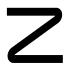
\includegraphics[keepaspectratio]{images/part001_e30b1f1b.jpg}}

The polynomial ring \(\mathbf{Q}[(\mathrm{X}_{n})_{n\in\mathbf{N}}]\) is an integral domain; it is not Noetherian (or Artinian) (VIII, p.~15, Exercise 9). It is a subring of its field of fractions, which is an Artinian (and Noetherian) ring.

